\section{Overview}
\hspace{0.5cm} This chapter defines aircraft performance characteristics and discusses the generalized range equation for jet aircraft and the simplifications known as the Br\'eguet range and endurance equations used by  Cavcar \cite{breguetRangeEqn}, Raymer \cite{LoiterTimeFromRange}, and Chuck et al. \cite{fuelsLOGRange} for design optimization as well as the incorporation of multiobjective optimization in flight optimization. The derivation of these equations rely on several key assumptions which define the flight plan of an aircraft and ascertain a conservative assessment of maximum range and endurance. Specifically, these equations rely on a constant thrust-specific fuel consumption ($TSFC$) and a constant lift over drag, which was used by Vitte \cite{OptimizeBreguet} for optimization of continuous target coverage and shown effective for evaluating the number of UAVs needed for a mission. Noteably, the range and endurance equations can be derived in terms of each other \cite{LoiterTimeFromRange}, making multiobjective optimization more useful if these two equations can be constrained by similar terms. 
\section{Aircraft Performance Characteristics}
Lift of a specific aircraft is generated by flight conditions and angle of attack. The lift coefficient depends on wing angle of attack, wing span, aircraft speed and other factors of the aircraft design including the fuselage, engine nacelles, and horizontal tail. Thus, any changes to angle of attack, speed, or design can impact the lift coefficient. \par
The total drag on an aircraft is influenced by speed, profile drag, and induced drag and varies based on lift. These are represented by a drag polar:
\begin{equation*}
    C_D = C_{D_0} + kC_L^2
\end{equation*}
where $C_D$ is total drag, $C_L$ is the coefficient of lift, and $C_{D_0}$ is the parasite drag coefficient and represents all drag generated by an aircraft when not experiencing lift. The constant $k$ is an expression where $k = 1/(\pi A_R e_0)$. $A_R$ is the aspect ratio of an aircraft and $e_0$ is the Oswald's efficiency factor for a three-dimensional wing's change in drag as compared to an ideal wing with the same aspect ratio. Since both parasitic drag and $k$ remain constant during flight, a change in the coefficient of lift will impact the coefficient of drag and vice versa with the added impact of mach number shown in Figure \ref{fig:clvscd}.
\begin{figure}[h] 
    \centering
    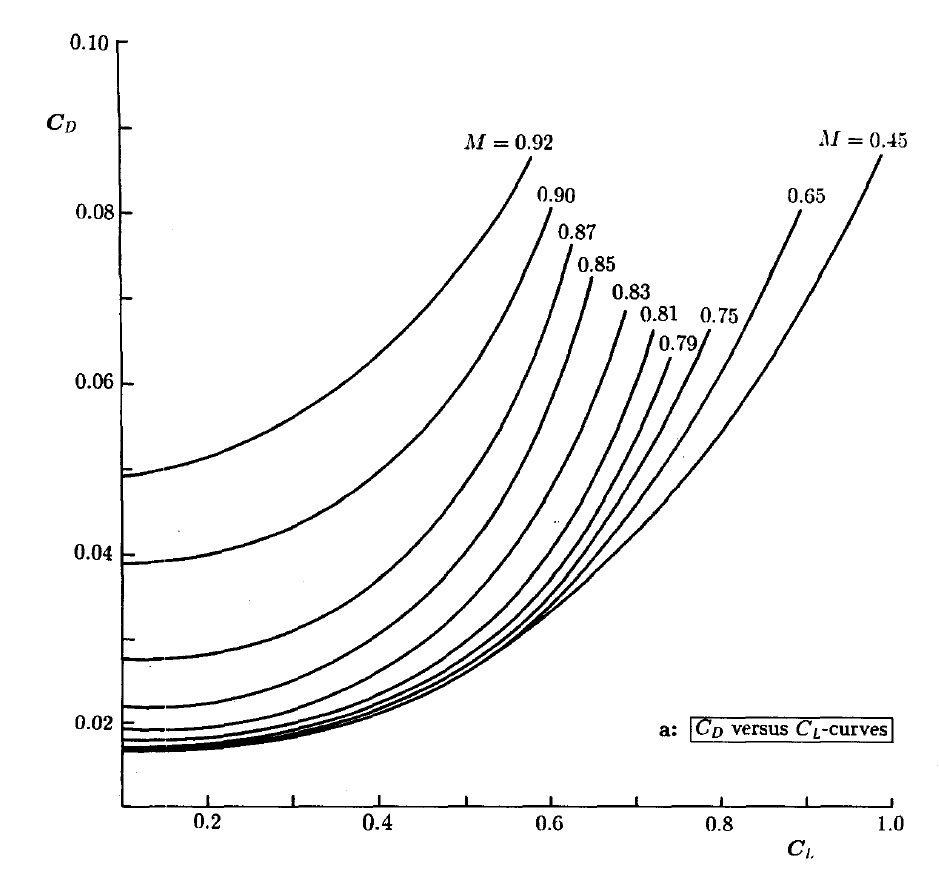
\includegraphics[width = 12cm]{Thesis/LiteratureReview/clvscd.PNG}
    \caption{Coefficient of Lift versus Coefficient of Drag with Mach Number \cite{torenbeek}}
    \label{fig:clvscd}
\end{figure}
Generally, the aircraft becomes less efficient at a higher mach number which impacts the $C_L/C_D$ and in turn effects the maximum range and/or loiter time of the aircraft. \par
The production of thrust allows the aircraft system to be most suitable for specific flight regimes. There are two main characteristics of propulsion systems. The first is the ratio of an engine's sea level output to its own weight which is set for all aircraft examined in this research. The second is thrust-specific fuel consumption and is more interesting to the given problem. Thrust-specific fuel consumption ($TSFC$) is the ratio of fuel consumption to thrust output:
\begin{equation*}
    TSFC\equiv \dfrac{\dot{W}}{T}
\end{equation*}
where $\dot{W}$ is the rate of fuel consumption and $T$ is thrust output. This equation determines operating envelopes for mach number and an engine's maximum thrust-to-weight ratio. Additionally, thrust output is impacted by altitude and thus changes depending on the altitude of a flight profile.
\section{Br\'eguet's Range Equation}
\hspace{.5cm} Br\'eguet's range equation combines specific fuel consumption, lift, drag, cruising speed, and initial and final fuel weights with aircraft weight. The derivation of this equation starts with several steps that are important for the sake of assumptions used in each simplification. Eq. \ref{eqRangeEq} is integration over the change in weight to solve for distance. The integration for the change in weight does not account for changes in the flight characteristics of the aircraft such as lift over drag, velocity, and thrust-specific fuel consumption which are variable depending on weight. These can be generalized by assumptions or by integrating over small weight changes with given parameters. The in-depth derivation of these equations are discussed in Section \ref{section: derive equations}.
\begin{equation}
    R = \int_{W_f}^{W_i}\dfrac{VdW}{(TSFC)D}
    \label{eqRangeEq}
\end{equation}
where $V$ is the speed of the aircraft, $D$ is drag, and $W_i,W_f$ are the initial and final weight of the aircraft, respectively. \par 
Assuming constant altitude, constant angle-of-attack, and constant thrust specific fuel consumption, the equation simplifies to Eq. \ref{eqBreguet}.
\begin{equation}
\label{eqBreguet}
R = \sqrt{\dfrac{2}{\rho_\infty S}}\left(\dfrac{1}{TSFC}\right) \left(\dfrac{C_L^{1/2}}{C_D}\right)(\sqrt{W_i}-\sqrt{W_f})
\end{equation}
where $\rho_\infty$ is the atmospheric density at altitude, $S$ is the wing area, and $C_L/C_D$ is the coefficient of lift over coefficient of drag. The simplicity of this equation lends itself well to optimization of more complex problems. \par 
If, however, the assumption for constant altitude is relaxed, but constant airspeed is assumed, the equation relies on fewer constants and becomes Eq. \ref{eqAirspeedAOA}.
\begin{equation}
\label{eqAirspeedAOA}
    R = \dfrac{V}{TSFC}\left(\dfrac{C_L}{C_D}\right)\ln\dfrac{W_i}{W_f}.
\end{equation}
Chuck et al. \cite{fuelsLOGRange} use Eq. \ref{eqAirspeedAOA} to compare fuel design effects on range. Mostly due to its logarithmic design, this equation accounts for fuel efficiency in that as an aircraft burns fuel, the lighter the aircraft becomes and thus can travel farther. This makes the use of this equation more realistic for longer enduring aircraft. \par
The final well-established derivation of the range equation is the equation assuming a constant airspeed, constant altitude, and parabolic drag polar. A parabolic drag polar more closely mimics the drag of an aircraft during flight and fuel burn than assuming constant drag in previous equations. Eq. \ref{eqDragPolar} shows the result of these assumptions on Eq. \ref{eqRangeEq}. The equation assumes that there is an initial coefficient ($C_{L_1}$) of lift and final coefficient of lift ($C_{L_2}$) with a coefficient of lift for maximum range ($C_{L_{MR}})$.
\begin{equation}
\label{eqDragPolar}
    R = \dfrac{2V}{TSFC}\left(\dfrac{L}{D}\right)_{max}\left[\arctan\dfrac{C_{L_1}}{C_{L_{md}}}-\arctan\dfrac{C_{L_2}}{C_{L_{md}}}\right]
\end{equation}
where $C_L/C_D = L/D$. The main limitation of this equation is the inability to project an aircraft into future space with limited given parameters such as a drag polar.\par
The assumption that lift and drag are constant can simplify the coefficients of lift and drag for maximum range. Eqs. \ref{eq:maxlift} and \ref{eq:maxdrag} illustrate these simplifications as shown in the basic performance equation introduced by \cite{OptimizeBreguet}.
\begin{equation}
C_{L_{MR}} = \sqrt{\dfrac{C_{D_0}}{3k}}
\label{eq:maxlift}
\end{equation}
\begin{equation}
C_{D_{MR}} = \dfrac{4}{3}C_{D_0}
\label{eq:maxdrag}
\end{equation}
where $C_{D_0}$ is parasitic drag and $C_{D_{MR}}$ is the coefficient of drag for maximum range. Jonas \cite{Jonas} argues that these equations are not accurate at predicting realistic results when accounting for changes in weight over the course of an aircraft's flight due to fuel burn. The new derivation of the range equation \cite{Jonas} where weight is dynamic produces the following equation:
\begin{equation}
    R = (b/a)[\arctan(W_i/a)-\arctan(W_f/a)].
    \label{eq:dynamicrange}
\end{equation}
The constants $a^2$ and $b$ are given by 
\begin{equation}
    \begin{aligned}
        a^2 &= \dfrac{C_0qS+C_1C_{D_0}(qS)^2}{k C_1}\\
        b &= \dfrac{VqS}{k C_1}
    \end{aligned}
\end{equation}
where $C_0$ and $C_1$ are constants for altitude and airspeed for a problem instance and $k = 1/(\pi A_R e)$. The results of these derivations were applied to a hypothetical jet \cite{Jonas}. The results showed a range only 0.77\% higher than the exact value obtained from the original range equation. The new method was considered accurate as compared to the Br\'eguet range equations and validated the use of aircraft and engine parameters available. This showed that regardless of the original hypothesis that the Br\'eguet range equation was an inaccurate depiction of true range, the Br\'eguet range equation performs well when compared against equations that use less assumptions.\par
As stated before, the weight change over time changes the fuel efficiency of an aircraft. Jonas \cite{Jonas} derives an equation involving the overall efficiency slope, $m$ that describes fuel efficiency. Eq. \ref{eqRangeIncludesM} shows the results of this derivation.
\begin{equation}
    R = \dfrac{aVJC_H}{10,560m}log_e\dfrac{W_i}{W_i-W_F}
    \label{eqRangeIncludesM}
\end{equation}
where $V$ is airspeed in feet per second, $J$ is a constant representing mechanical heat at 778.26 foot pounds per BTU, $C_H$ is the fuel heat value in BTU per pound, and $a$ is equivalent to $2C_L/C_D$. These values are not included in the available data for this research and so the most useful equation was derived by Jonas \cite{Jonas} shown in Eq. \ref{RangeChanges}.
\begin{equation}
    R = \dfrac{W_i}{1.467}\dfrac{V}{Q_I}\ln\dfrac{W_i}{W_i-W_f}
    \label{RangeChanges}
\end{equation}
where $Q_I$ is $\theta_f/\theta_i$ which is the ratio of altitude density over the course of the cruise. This equation is useful when reducing the assumptions in a flight plan since simplifying assumptions are made about the ratios between density, weight, and lift over drag. Eqs. \ref{eqRangeIncludesM} and \ref{RangeChanges} allow for the removal of the constant altitude assumption. These results were also compared to the original Br\'eguet range equation's simplifications using various assumptions for accuracy. \par
\section{Endurance Equation}
In addition to maximum range, loiter time is needed and relates to the endurance equation. Endurance is the calculated time that an aircraft can remain in the air. The general endurance equation is represented as
\begin{equation}
    \Delta t = \dfrac{\Delta W_f}{(TSFC)D}
\end{equation}
where $\Delta W_f$ is the change in weight due to fuel burn. Brandt \cite{IntrotoAero} introduces an average value method for this prediction as
\begin{equation}
    E = \dfrac{\Delta W_f}{(TSFC)D_{avg}}
\end{equation}
and states that the results for turbojet aircraft are often accurate, but the more accurate prediction of endurance is
\begin{equation}
    E = -\int_{W_i}^{W_f}\dfrac{dW}{(TSFC)D}.
\end{equation}
Assuming a constant angle of attack, similar to Eq. \ref{eqAirspeedAOA}, hence a constant $C_L$ and $L/D$ and noting that lift equals weight,
\begin{equation*}
    E = \int_{W_f}^{W_i}\dfrac{1}{TSFC}\dfrac{L}{D}\dfrac{dW}{W} = \dfrac{1}{TSFC}\dfrac{C_L}{C_D}\int_{W_f}^{W_i}\dfrac{dW}{W}
\end{equation*}
\begin{equation}
\label{endure}
    E = \dfrac{1}{TSFC}\left(\dfrac{L}{D}\right) \ln\left(\dfrac{W_i}{W_f}\right).
\end{equation}
Eq. \ref{endure} shows the final equation and for the remainder of the paper endurance, $E$, will be equivalent to loiter time.\par
The endurance equation's lift and drag elements can be replaced by an angle of attack for best endurance \cite{OptimizeBreguet} shown in equation \ref{eq:maxendurance}.
\begin{equation}
\label{eq:maxendurance}
\dfrac{L}{D} = \dfrac{C_{L_{ME}}}{C_{D_{ME}}} = \sqrt{\dfrac{1}{4KC_{D_0}}}
\end{equation}
where $C_{L_{ME}}/C_{D_{ME}}$ is the coefficient of lift over coefficient of drag for maximum endurance. This is important for an aircraft to maximize its potential when performing a maneuver. However, the assumption that this is constant requires that the aircraft fly slower as weight decreases. The combination of the average value method and the assumptions for Eq. \ref{endure} is the approximation method utilized for testing the methodology.
\par 
The simplification of these equations involves introducing an unknown amount of error into a continuous problem. There are analytical solutions to reduce this error shown by Vitte \cite{OptimizeBreguet} and Raymer \cite{LoiterTimeFromRange}. These give insight into the differences between using the endurance and range equation for a discrete set of weights versus a continuous set of weights. Raymer \cite{LoiterTimeFromRange} uses the non-linear Br\'eguet range equation to approximate the maximum loiter time of an aircraft. Employing approximate conditions of cruise $(L/D)$ versus loiter $(L/D)$, Raymer \cite{LoiterTimeFromRange} finds that 
\begin{equation}
    \dfrac{R_{cruise}}{V_{cruise}} = \dfrac{TSFC_{loiter}}{TSFC_{cruise}}\dfrac{(L/D)_{cruise}}{E_{loiter}}
\end{equation}
where $E_{loiter}$ is the loiter time. Finding the approximate relationship between the $(L/D)$s of both loiter and cruise made Raymer's method approximately $5\%$ optimistic when compared to tested jets and shows that the results are accurate when equating loiter time to endurance.
\section{Multiobjective Optimization}
Pareto introduced the concept of dominated solutions in the field of economics in 1906 to describe a solution that best serves all parties in a multiplayer game \cite{paretomanual}. A Pareto efficiency is defined as a state where a reallocation of products to any party where this party is better off to the detriment of at least one other party. A Pareto frontier is the set of these pareto efficiencies. Economics and engineering have coordinated this concept into design and performance optimization \cite{surveyMarler}. A Pareto frontier in an aircraft's performance space can be readily visualized when there are few objectives. In this case, two objectives gives a reasonable expectation for a straightforward visualization. Agrawal et al. \cite{MultiobjectiveVisualization} use an initial mapping from a design space to a performance space in multiple dimensions and proves that the visualization using performance is a better method for an $n$-dimensional design space. However, the performance space of the Pareto frontier proposed in this paper is only two-dimensional and does not require the complicated mapping of a design space to a performance space from multiple dimensions. 
\par
Korhonen et al. \cite{MultOptCS} point out that there are two main methods when approaching a multiobjective optimization problem. These are the weighting method and the constraint method. In these two methods, the decision maker can control the solution process with their preferences.\par
\subsection*{Weighting Method}
The weighting method involves solving the following multiobjective optimization problem,
\begin{equation}
\begin{aligned}
    &\min \sum^k_{i=1} w_if_i(\mathbf{x})\\
    &\hbox{subject to} \ \mathbf{x}\in S,
\end{aligned}
\label{eq:weightEq}
\end{equation}
where $w_i\geq 0 \ \ \forall i = 1,\dots,k$ and each objective is normalized so that magnitudes are not a factor in the solutions. By using multi-objective optimization, the analyst can weight one function as important over another over a tradeoff region and explore the Pareto frontier of solutions. The solution to Eq. \ref{eq:weightEq} is weakly Pareto optimal and not necessarily unique. The solution is Pareto optimal if for all $i = 1,\dots,k$, $w_i>0$ such that the solution is unique \cite{MultOptCS}. The weighting method can be used as a decision tool to generate different Pareto optimal solutions for the decision maker to choose from. The main requirement for the use of a weighting method is a convex problem. The optimal solutions of some nonconvex problems can sometimes be found no matter the weights, but cannot be proven and does not always behave like the convex solution method \cite{MultOptCS}.\par
\subsection*{$\epsilon$-Constraint Method}
The second method is the $\epsilon$-constraint method where one of the objective functions is optimized and the rest are used as constraints in the optimization problem. The form of this problem can be seen in Eq. \ref{eq:constraintEq}.
\begin{equation}
    \begin{aligned}
    \text{minimize} \ & f_i(\mathbf{x})\\
    \text{subject to} \ & f_j(\mathbf{x})\leq \epsilon_j, \hspace{0.5cm} \forall j = 1,\dots,k, \ j\neq l,\\
    & \mathbf{x}\in S.
    \end{aligned}
    \label{eq:constraintEq}
\end{equation}
\par
The $\epsilon$-constraint method is preferable for this research problem since only two objectives are examined. Additionally, since they share similar parameters, the constraint of one objective will subsequently optimize the second objective. The weighting method is unnecessarily complicated for the research method given its dimension, but is applicable to the optimization problem in Section \ref{section:DDF} for two objectives that are not dependent on similar parameters.

\section{Conclusion}
The Br\'eguet equations are a reliable way to define the range and endurance of an aircraft, given specific parameters. Additionally, the similarities between the range and endurance equation are used to define a tradeoff region for multiobjective optimization of range and loiter time. The next chapter will define a methodology of how these equations are formulated to allow for a tradeoff region and how each parameter is extracted from aircraft profiles.